\section{Data Deduplication}
\label{DD}

Data deduplication provides a means to efficiently remove redundancies from large datasets.
This process is made possible by first dividing up the data into segments and representing each segment with a much smaller hash value.
A redundant segment of data is then easily identified through a hash table lookup.
The efficiency of the process comes at the cost of possible data loss through hash collisions, thoug it is understood that the collision probability is negligible compared to the soft error rate of the storage system if an appropriate hash function is used~\cite{aronovich:2009, zhu:2008, bobbarjung:2006, muthitacharoen:2001}.
Another performance factor is the granularity of compression which is limited to the size of duplicate segments.
Two segments that are off by a single bit will result in no compression.

Despite these costs, data deduplication has steadily gained its place in backup~\cite{meister:2009, lillibridge:2009, zhu:2008}, archive~\cite{you:2005} and virtual machine storage solutions~\cite{smith:2008, jin:2009, clements:2009} due to its potentially huge reduction in storage space and IO elimination.

\begin{figure}[!t]
\centering
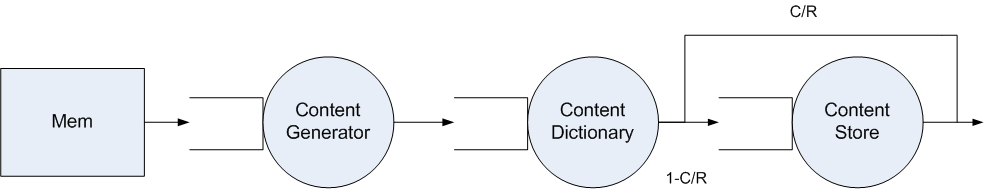
\includegraphics[width=3.5in]{figure/dedup/queue}
\caption{Our simplified deduplication system model. It is essentially 3 server open queuing system. At the content dictionary, C/R of the segments exit the system and 1-C/R of the segments are passed on to content store. All data are assumed to be immediately available at the memory and all three servers have exponentially distributed service time.}
\label{queue}
\end{figure}

%dedup component
The deduplication process itself can be divided into largely three parts as shown in \figurename~\ref{queue}. First part of the process generates a sequence of segments from input data stream which we call the \emph{content generator}. In the second phase, the deduplication system generates a dictionary of segments which is in turn used to identify the duplicate segments which we call the \emph{content dictionary}. In the last phase, new segments are stored on a persistent storage system which we call the \emph{content store}. The later two components form a \emph{content addressable storage}(CAS).

\subsection{Content Generator}
The goal of the content generator is to maximize the redundant segments while minimizing the number of segments generated.
These two goals often conflict with each other since the amount of duplicate data tends to increase with smaller segments size.
This is due to the fact that the generation of segments are typically done in stateless manner to keep up with the huge data size and stringent throughput requirements.
Recent papers try to overcome this limitation through a two level definition of contents~\cite{kruus:2010, bobbarjung:2006}.
However, these approaches come at the extra computation cost and are applicable only when there are less stringent throughput requirements.

%segmentation types
These are the three most common methods to define the segment boundaries also known as the \emph{anchors}~\cite{zhu:2008, muthitacharoen:2001}.
\begin{itemize}
  \item \emph{File based}: A file boundary becomes the segment boundary.
  \item \emph{Size based}: The anchors are designated every $k$ bits which determines the boundaries for the segment. Therefore, any addition or deletion of data results in shifted anchors which is propagated until the end of the data stream. This effect is known as the \emph{boundary shifting problem}~\cite{muthitacharoen:2001}.
  \item \emph{Content based}: An anchor is generated based on the content of the data which becomes the boundaries for the segments. Therefore the anchors are shifted together with the contents in the case of addition and deletion of the data.
\end{itemize}

The \emph{content based} approach is the most popular method used in data deduplication due to the boundary shifting problem found in the size based method.
Average, maximum and/or minimum segment size are usually specified for the content based approach. This allows system to expect segments of the bounded size which makes the segment handling simpler but also ensures that amount of size variation is limited which can cause loss of redundancy~\cite{eshghi:2005}.

%decoupling from the rest of the system
From the system perspective, the content generator is the source generator for the CAS. Typically, any information about the original data stream is lost after this point. This justifies our looking the dataset as a sequence of segments since beyond this point, the system is effectively decoupled from the original dataset.

\subsection{Content Dictionary}
%hash
The content dictionary is typically a hash table which is keyed by hash of segments. Hash functions used typically provide one-way property as well as collision resistance. While only the collision resistance is required for correct functionality, one-way property is also attractive to ensure that the malicious users cannot corrupt the system by generating hash collisions.

For a large dataset, the content store itself becomes significantly large.
To relax the memory requirements for the deduplication system, the content dictionary is typically stored on the disk~\cite{mandagere:2008, lillibridge:2009, zhu:2008, bhagwat:2009} .
Only a portion is cached onto the memory at a time. Furthermore, any writes to the index table must be serialized which require expensive locks~\cite{clements:2009}. Therefore, the caching algorithm for the index table is one of the major performance factor within the deduplication system.

To avoid unnecessary accesses to the index table, Bloom filter~\cite{bloom:1970} is used to quickly determine segments that are not in the index table~\cite{zhu:2008}. While the backup stream typically exhibit an inherent spatial locality between the segment instances~\cite{zhu:2008}, more intelligent caching schemes that uses data similarities have also been proposed~\cite{lillibridge:2009, bhagwat:2009}.

Regardless of caching scheme, it is clear that content dictionary determines the data path for any given segment. While every segment must read the index table at least once, only the new segments result in it's update. Furthermore, these new segments must be passed down to the content store to be store on the disk. Problem is more complicated for the read where segments maybe fragmented in various places both for the actual contents and the dictionary. A recent work duplicated heavily used segments over the physical disk such that the average seek time can be minimized~\cite{koller:2010}. However, such approach assumes small working set of segments and is heavily workload dependent.

In this work we assume nothing about the caching policy of the content dictionary or any other auxiliary data structure to minimize the access to the dictionary. We only assume that the different segment types results in different resource requirements in regular read/write operations.

\subsection{Content Store}

Once the segments are identified as new content that needs to be stored, it is passed down to the content store to be processed. Various different mechanisms are possible. The content may already be on the disk and the content store only generates a logical mapping and freeing of segments~\cite{clements:2009, rhea:2008} or use log-based filesystem to optimize for the in-band writes~\cite{zhu:2008}.

The content store is not affected specifically by the deduplication system. While inherent \emph{copy-on-write} (COW) support of storage subsystem~\cite{bonwick:2003, dillon:2008} allows easier sharing of segments, the fundamental operations of underlying storage does not differ from dataset to dataset. Therefore, we focus mostly on the behaviors of the content dictionary in this paper.

